\begin{document}

\begin{wrapfigure}{r}{0.5\textwidth}
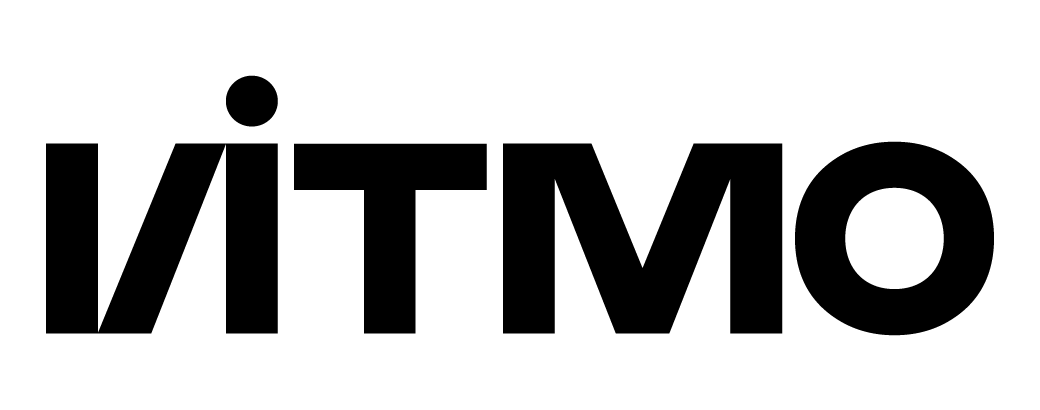
\includegraphics[width=0.6\linewidth]{fig/itmo.png}
\end{wrapfigure}


\centering\textbf{Университет ИТМО} \\
\centering\textbf{Физико-технический мегафакультет} \\
\centering\textbf{Физический факультет} \\ [0.5cm]


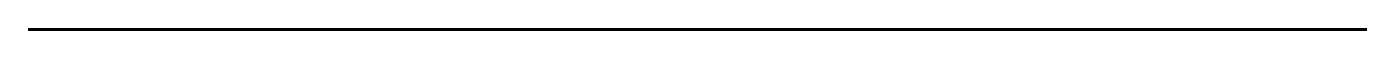
\begin{tikzpicture}
\path[fill=black,even odd rule] (0,0) rectangle (17.005,-0.036);
\end{tikzpicture}

\begin{tabular}{l l}
\TextField[name=group,color=black]{Группа} 
& \TextField[name=towork,color=black]{К работе допущен} \\
\TextField[name=student,color=black]{Студент}
& \TextField[name=workcomplete,color=black]{Работа выполнена}\\
\TextField[name=tutor,color=black]{Преподаватель} 
& \TextField[name=reportacc,color=black]{Отчёт принят}  \\[2cm]
\end{tabular}

\huge{\textbf{Рабочий протокол и отчёт по лабораторной работе {\textnumero}{\num}}}
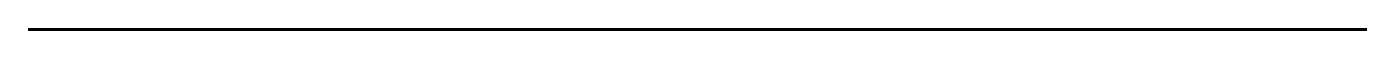
\begin{tikzpicture}
\path[fill=black,even odd rule] (0,0) rectangle (17.005,-0.036);
\end{tikzpicture}

\centering\Large\textbf{\labname}

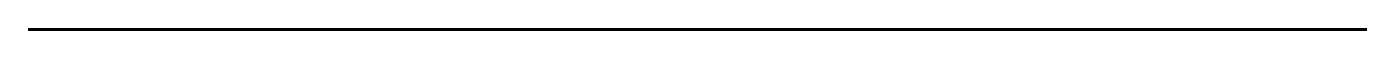
\begin{tikzpicture}
\path[fill=black,even odd rule] (0,0) rectangle (17.005,-0.036);
\end{tikzpicture}


\begin{flushleft}
\section{Цель работы.}
Цель работы

\section{Задачи, решаемые при выполнении работы.}
Задачи

\section{Объект исследования.}
Объект

\section{Метод экспериментального исследования.}
Метод

\section{Рабочие формулы и исходные данные.}
Формулы

\section{Измерительные приборы.}
\small
\begin{tabular}{|c|c|c|c|}
    \hline
    \textit{№ п/п} 
     & \textit{Наименование} 
     & \textit{Диапазон значений}
     & \textit{Погрешность прибора} \\
     \hline
     1. & Название прибора & Диапазон & Погрешность\\
     \hline
\end{tabular}

\section{Схема установки (\textit{перечень схем, которые составляют Приложение 1}).}


\section{Результаты прямых измерений и их обработки (\textit{таблицы, примеры расчетов}).}

\section{Расчет результатов косвенных измерений (\textit{таблицы, примеры расчетов}).}

\section{Расчет погрешностей измерений (\textit{для прямых и косвенных измерений}).}

\section{Графики (\textit{перечень графиков, которые составляют Приложение 2}).}


\section{Окончательные результаты.}


\section{Выводы и анализ результатов работы.} 

\section{Дополнительные задания.}
\bigskip

\section{Выполнение дополнительных заданий.}. 
\section{Замечания преподавателя (\textit{исправления, вызванные замечаниями преподавателя, также помещают в этот пункт}).} 


\bigskip
\end{flushleft}
\end{document}
